\documentclass[usenames,dvipsnames,aspectratio=169,table]{beamer}
%\usetheme{cern}
\usetheme{cernomc}

\usepackage{scrextend}
\changefontsizes{8pt}

% Beamer Setup ---
\setbeamercovered{transparent=5} 
\setbeamertemplate{navigation symbols}{} 

\AtBeginSection{%
	\begin{frame}[noframenumbering]{Outline}
	\tableofcontents[currentsection]
	\end{frame}
}

% Imports ---
\usepackage[utf8]{inputenc}
\usepackage{amsmath}
\usepackage{amsfonts}
\usepackage{amssymb}
\usepackage{unicode-math}
\usepackage{mathtools}
\usepackage{bm}  % bold math
\usepackage{graphicx}
\usepackage{grffile}  % filenames with dots 
\usepackage{fontawesome5}
\usepackage{minted}

\usepackage{tikz}
\usetikzlibrary{calc}

\usepackage{hyperref}
\usepackage{siunitx}
\usepackage{booktabs}
\usepackage{multirow}
\usepackage{caption}
\usepackage[absolute,overlay]{textpos}

\usepackage{fontspec}
\usefonttheme{serif}
%\setmainfont{STIX Two Text}
%\setmathfont{STIX Two Math}
\setmainfont{TeX Gyre Bonum}
\setmathfont{TeX Gyre Bonum Math}
\setmonofont{Fira Code}


% some shenanigans -------------------------------------------------------------
\newcommand{\highl}[1]{\textbf{#1}}
\definecolor{RunTwored}{RGB}{200,0,0}
\definecolor{APJgreen}{RGB}{20,150,0}
\definecolor{SbSorange}{RGB}{240,150,0}
\newcommand{\we}{\cellcolor{blue!20!white}}
\newcommand{\ho}{\cellcolor{red!20!white}}
\newcommand{\wh}{\cellcolor{green!20!white}}
\newcommand{\bonelabel}{%
        \node at ($(b1) +(-0.13\linewidth, 0.15\linewidth)$) {\sffamily\small\textbf{Beam 1}};
}
\newcommand{\btwolabel}{%
        \node at ($(b2) +(-0.13\linewidth, 0.15\linewidth)$) {\sffamily\small\textbf{Beam 2}};
}

\renewcommand{\theFancyVerbLine}{\textcolor[rgb]{0.5,0.5,1.0}{\scriptsize\arabic{FancyVerbLine}}}


% Meta -------------------------------------------------------------------------
\author[awegsche]{%
Andreas Wegscheider\\[1em]
\centering%

\includegraphics[width=3cm]{OMC_logo_original.pdf}%
}
\title[Magnet sorting]{Magnet sorting strategy}
\logo{} 
\titlegraphic{}
\institute{CERN}
\date[18.10.23]{18.10.2023}
\subject{} 

% Document ---------------------------------------------------------------------
\begin{document}

\begin{frame}
    \titlepage
\end{frame}


%\begin{frame}{Full Outline}
%\tableofcontents
%\end{frame}

%\section{Lobster Measurements}

\begin{frame}[fragile]
    {Current status}


    \begin{minipage}{0.45\linewidth}
    \begin{itemize}
        \item setup simulation scripts to \highl{introduce errors} and \highl{control sorting}\\
        \item ran extensive simulations with \highl{naive} sorting methods
        \item recorded correctability using omc3's \texttt{global\_correct}
    \end{itemize}
    \end{minipage}
    \hfill
    \begin{minipage}{0.52\linewidth}
        Example usage:
        \small
        \begin{minted}
            [
            xleftmargin=1em,
            fontsize=\footnotesize,
            linenos,
            bgcolor=blue!5!white,
            auto
            ]
            {python}
q2_errors = Q2Pairs(real_errors=10,
                    meas_errors=2,
                    stage=1)

# apply sorting on sum
q2_errors.sort_sum()

# write errors to madx file
q2_errors.write_errors_to_file("errors_Q2.madx")

# run madx, run global_correct, compare outputs
# ...
        \end{minted}
    \end{minipage}
\normalsize
    
\end{frame}

\begin{frame} % ------------------------------------------------------------------------------------
    {Effect on correctability}


    \textbf{Note} Left: only Q2 sorting/pairing is considered, according to the possibilities in Ezio's document.

    Plots show relative $\beta$~beating after correction, before and after sorting.
    
    
    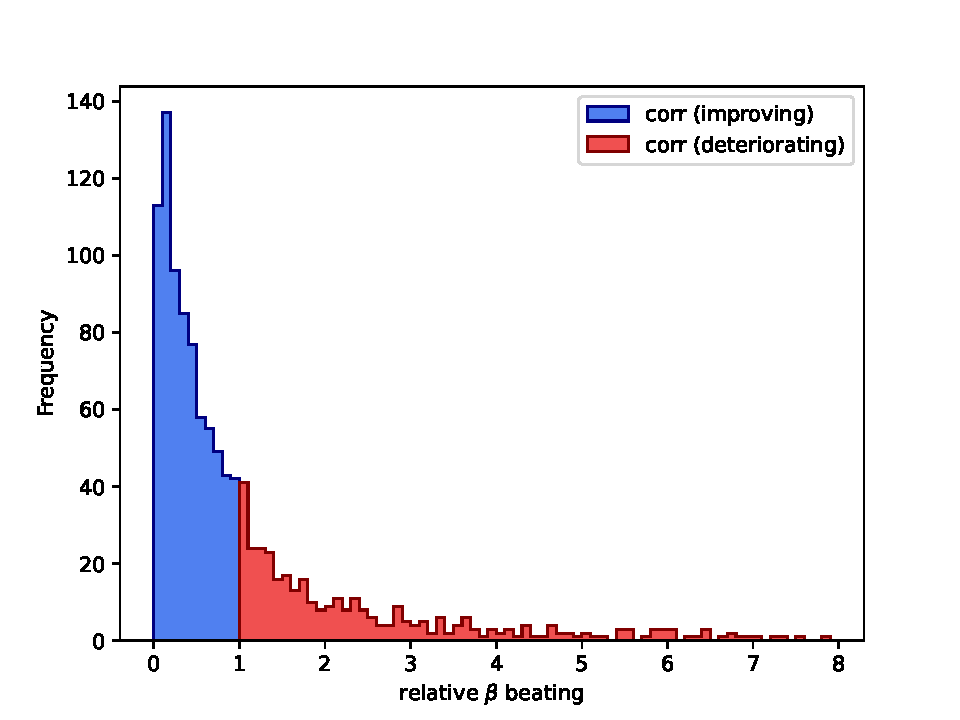
\includegraphics[width=0.45\linewidth]{corr_onlyQ2.pdf}
    \hfill
    \includegraphics[width=0.45\linewidth]{corr_both.pdf}

    Statistics for sorting at all stages will come soon.

\end{frame} % --------------------------------------------------------------------------------------


\begin{frame} % ------------------------------------------------------------------------------------
    {Correlation}

    \begin{minipage}{0.6\linewidth}
        \includegraphics[width=\linewidth]{correlation_both.pdf} 
    \end{minipage}
    \begin{minipage}{0.39\linewidth}
        improvement in correctability is slightly correlated to initial improvement in $\beta$~beating 
    \end{minipage}
    
\end{frame} % --------------------------------------------------------------------------------------


\begin{frame} % ------------------------------------------------------------------------------------
    {Current work / future plans}


    \begin{itemize}
        \item develop more sophisticated sorting methods (optimise transfer matrices, ...)
        \item check sorting / pairing for different stages of the assembly process
        \item check other correction methods (SbS, APJ)
    \end{itemize}
    
\end{frame} % --------------------------------------------------------------------------------------
% \backcover

\begin{frame}[fragile]
        \begin{minted}
            [
            fontsize=\footnotesize,
            linenos,
            bgcolor=blue!5!white,
            ]
            {python}
q2_errors = Q2Pairs(real_errors=10,
                    meas_errors=2,
                    stage=1)

# apply sorting on sum
q2_errors.sort_sum()

# write errors to madx file
q2_errors.write_errors_to_file("errors_Q2.madx")

# run madx, run global_correct, compare outputs
# ...
        \end{minted}

\end{frame}

\end{document}
